\documentclass[../../Main/Apputni Fisica.tex]{subfiles}
\begin{document}
\begin{figure}[!h]
    \centering
    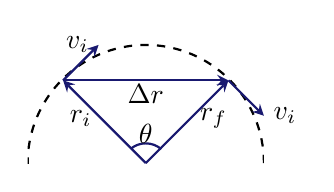
\begin{tikzpicture}[scale = 1, every node/.style={scale=1}]

        % Circular motion trajectory
        \begin{scope}
            \clip (-1.5, 0) rectangle (1.5, 1.6);

            \draw[dashed, thick] (0, 0) circle (1.5);

        \end{scope}
        % Velocity and position vectors
        %% Position
        \draw[-stealth, thick, MidnightBlue] (0, 0) -- (1.05, 1.05);
        \node (r_f) [anchor = west] at (0.565, 0.565) {\(\va{r_{f}}\)};

        \draw[-stealth, thick, MidnightBlue] (0, 0) -- (-1.05, 1.05);
        \node (r_i) [anchor = east] at (-0.565, 0.565) {\(\va{r_{i}}\)};

        \draw[-stealth, thick, MidnightBlue] (-1.05, 1.05) -- (1.05, 1.05);
        \node (Delta r) [anchor = north] at (0, 1.125) {\(\vb{\Delta r}\)};

        %% Velocity
        \draw[-stealth, thick, MidnightBlue] (-1.05, 1.05) -- (-0.6, 1.5);
        \node (v_i) [anchor = east] at (-0.6, 1.5) {\(\va{v_{i}}\)};

        \draw[-stealth, thick, MidnightBlue] (1.05, 1.05) -- (1.5, 0.6);
        \node (v_i) [anchor = west] at (1.5, 0.6) {\(\va{v_{i}}\)};

        % Angle between r_i and r_f
        \draw[thick, MidnightBlue] (0, 0.25) arc(90:49:0.3);
        \draw[thick, MidnightBlue] (0, 0.25) arc(90:129:0.3);

        \node (theta) [anchor = south] at (0, 0.125) {\(\theta\)};

    \end{tikzpicture}
    \caption{TODO}
    \label{fig:3}
\end{figure}
\end{document}